\documentclass[tikz,border=8pt]{standalone}
\usetikzlibrary{decorations.pathreplacing}
\begin{document}
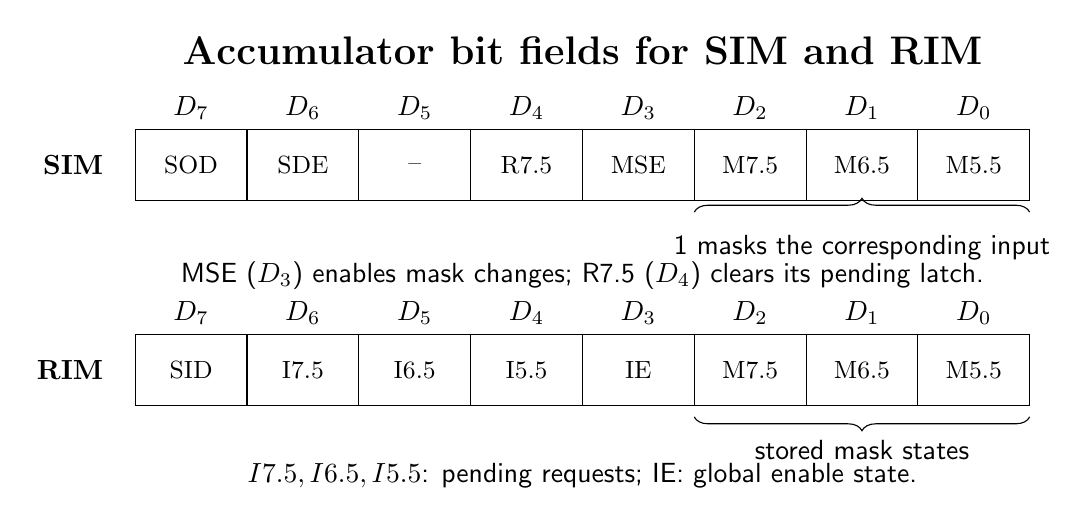
\begin{tikzpicture}[font=\sffamily,x=1.42cm,y=1cm]
\node[font=\Large\bfseries] at (4,5.55) {Accumulator bit fields for SIM and RIM};
\foreach \x in {0,...,8}{\draw (\x,3.65) -- (\x,4.55); \draw (\x,1.05) -- (\x,1.95);}
\draw (0,3.65) rectangle (8,4.55);
\draw (0,1.05) rectangle (8,1.95);
\foreach \x/\b in {0/7,1/6,2/5,3/4,4/3,5/2,6/1,7/0}{
  \node[above] at (\x+.5,4.55) {$D_{\b}$};
  \node[above] at (\x+.5,1.95) {$D_{\b}$};
}
\foreach \x/\s in {0/SOD,1/SDE,2/--,3/R7.5,4/MSE,5/M7.5,6/M6.5,7/M5.5}{\node[font=\small] at (\x+.5,4.1) {\s};}
\foreach \x/\s in {0/SID,1/I7.5,2/I6.5,3/I5.5,4/IE,5/M7.5,6/M6.5,7/M5.5}{\node[font=\small] at (\x+.5,1.5) {\s};}
\node[left,font=\bfseries] at (-.2,4.1) {SIM};
\node[left,font=\bfseries] at (-.2,1.5) {RIM};
\draw[decorate,decoration={brace,amplitude=5pt}] (5,3.5)--(8,3.5) node[midway,below=5pt] {1 masks the corresponding input};
\draw[decorate,decoration={brace,amplitude=5pt,mirror}] (5,.9)--(8,.9) node[midway,below=5pt] {stored mask states};
\node[align=center] at (4,2.7) {MSE ($D_3$) enables mask changes; R7.5 ($D_4$) clears its pending latch.};
\node[align=center] at (4,.15) {$I7.5,I6.5,I5.5$: pending requests; IE: global enable state.};
\end{tikzpicture}
\end{document}
